\documentclass[10pt,twocolumn]{article}
\usepackage[a4paper,margin=15mm]{geometry}
\usepackage{amsmath,amssymb}
\usepackage{amsthm}
\usepackage{graphicx}
\theoremstyle{plain}
\newtheorem{theorem}{Theorem}
\newtheorem{lemma}[theorem]{Lemma}
\newtheorem{proposition}[theorem]{Proposition}
\newtheorem{corollary}[theorem]{Corollary}
\theoremstyle{remark}
\newtheorem{remark}[theorem]{Remark}
\usepackage{booktabs,array,calc}
\usepackage[font=small,labelfont=bf]{caption}
\usepackage[colorlinks=true]{hyperref}
\providecommand{\tightlist}{\setlength{\itemsep}{0pt}\setlength{\parskip}{0pt}}
\emergencystretch=3em
\allowdisplaybreaks

\begin{document}
\title{Regime Viability on the Northern Cod Stock:\\
An Exact Certification of Obstruction Structure\\
on Public Assessment Data}
\author{Amin Abaee\\[0.35em]
{\small Independent Researcher}\\[0.55em]
{\small\href{https://orcid.org/0000-0002-0019-1842}{ORCID: 0000-0002-0019-1842}}\\[0.3em]
{\small\href{mailto:amin\_abaee@ut.ac.ir}{amin\_abaee@ut.ac.ir}}}
\date{September 26, 2026}
\maketitle

\begin{abstract}
The viability machinery of the obstruction calculus has been developed
and validated on deliberately small exact instances. This paper applies
it to a real assessment record --- the Northern cod stock (NAFO 2J3KL),
read from the published assessment input series, the 2025 reassessment
series, the official removals tables, the long-duration catch
reconstruction, the research-vessel survey index, and an independently
monitored forage-fish covariate --- and certifies, in exact rational
arithmetic, the obstruction structure that the historical collapse
exhibited. The certified object is a \emph{harvest-free multiplier
bracket}: for each annual step, the interval's per-capita non-fishing
growth factor lies in
\(\bigl[\rho,\ \max\{\rho+r,\ \rho/(1-r)\}\bigr]\), where \(\rho\) is
the realized net multiplier and \(r\) the removals fraction, under
either timing convention for the removals accounting. Both collapse
steps certify as harvest-free contractions under every convention
(upper bounds \(0.754\) and \(0.372\)); the reference window's worst
step and the two prelude steps do not certify (brackets straddle
unity) --- a typology, not a blanket verdict. Under the post-moratorium
removals rows (\(1{,}314\) and \(413\) t, at most \(1.4\%\) of the
stock), the brackets certify continued contraction, and the stock fell
by a factor of \(\tfrac{10105}{968} \approx 10.4\) in two years to its
series minimum. The \(276\) kt auxiliary floor separates the reference
window from the collapse era without exception, while the
\(884.6\) kt reference point --- the window's own mean --- has three of
the seven window readings below it in sample and therefore separates
nothing. Three extensions certify robustness and scope: on the
reassessment vintage's published 95\% bands, exactly the four
collapse-era steps 1991--1995 certify as declines and the 1993 floor
breach holds at the band's upper edge (\(115 < 276\)), while no
reference-decade step certifies; the reference decade's window profile
shows every subwindow of horizon four or more growing (the sustained-decline
reading holds only at horizons one to three); and the vintage's own
1954--1982 record has the window opening at \(28.3\%\) of the 1962 peak,
three years after a prior floor episode (1977--1979). The collapse is present in the raw survey index (a certified
factor of \(\tfrac{21797}{2127417}\) over 1989--1994, falling \(2.6\)
times further than the assessment series over their common window);
the forage-fish covariate collapses in the same annual step in which
the mortality diagnostic crosses \(M=1\), two steps before the floor
breach; and both assessment vintages re-cross the floor at the 2015
reading, with outcome years at most
\(\tfrac{44000}{88460} \approx 49.7\%\) of the reference point. Every
quantity is regenerated by an accompanying verification script in
exact rational arithmetic.
\end{abstract}

\textbf{Keywords:} viability; obstruction; regime shift; Northern cod;
exact computation; monitoring design; limit reference points

\section{Introduction}\label{intro}

The viability and obstruction machinery of the calculus --- survivable
sets, robust multipliers, breach-time certificates, and probe design ---
is developed in Abaee (2026a) and validated on deliberately small exact
instances. This paper applies it to the Northern cod stock (NAFO
divisions 2J3KL) --- the running record of this paper --- and certifies
the obstruction structure of its collapse on the public assessment
record. The forecast layer of the
same record --- the scoring of competing forecast ladders and the
2022--2023 observation suspension as a review-timing event --- is
certified in a companion paper (Abaee, 2026c, Section 3.10); the
present paper certifies the viability layer. The two are companions by
construction: the forecast ladder prices what can be predicted, this
paper prices what could have been kept safe.

The claims below are of three kinds, and the label travels with the
claim. \emph{Arithmetic claims} are exact rational identities or
inequalities on the certified rows; they are regenerated by the
verification script and cannot drift. \emph{Provenance claims} state
which file, which vintage, and which column a number comes from, and
whether that column is a model input or a model output. \emph{Scope
claims} are conditional readings --- stress bounds, sustained
hypotheticals, design critiques --- and are labelled as such where
they appear. No claim of the first kind rests on an interpretation; no
claim of the third kind is stated as one of the first. The
contributions are: the record spine --- the certified 1960--2023
assessment-record reconstruction with its provenance ledger (Sections
\ref{spine}--\ref{windows}); the harvest-free multiplier brackets ---
the exact two-form accounting bracket isolating the non-fishing growth
factor (Section \ref{brackets}); and the window profile and band
certificates --- the collapse's obstruction structure certified on the
public record, with the certified-record figure reading every annotated
value from the locked files (Section \ref{profile}).

\section{Data and provenance}\label{data}

Seven locked public files are used, each cross-verified against its
primary source at archival time (Abaee, 2026d): (i) the NCAM (Northern Cod Assessment Model) 2016
assessment input series (DFO, 2016, Table A2): spawning stock biomass
in kilotonnes, 1983--2015, cross-checked 33 of 33 years against the
primary report --- the \emph{input vintage} of the biomass record;
(ii) the xteNCAM 2025 reassessment SSB series (Regular et al., 2025,
Table 17), 1954--2024, with 95\% bands and SSB-over-\(B_{\mathrm{lim}}\)
ratios --- the \emph{reassessment vintage}; (iii) the official
removals table (Regular et al., 2025, Table 1), 1954--2023; (iv) the
catch reconstruction (Schijns et al., 2021, Table 1); (v) the fall
research-vessel survey abundance index (Schijns et al., 2021, Table 3,
citing DFO 2021b) --- a research-vessel input to the assessments, not
an output of them; (vi) the RAM Legacy database per-year extract for
this stock (free, 2024 release), 1850--2021 --- the \emph{database
vintage}, extending the series to 2021; and (vii) the capelin acoustic
biomass series (observed years only, no interpolation).

Two thresholds appear throughout, and their provenance is stated once
here. The \emph{auxiliary floor} \(B_{\mathrm{aux}} = 276\) kt is the
reassessment vintage's \(B_{\mathrm{lim}}\) at the file's rounding: the
published ratio column is rounded to two decimals, and the values it
implies for \(B_{\mathrm{lim}}\) range from \(250\) to \(289\) kt
across the file's years. Every floor comparison below is insensitive
across that range (the compared quantities clear it by large factors;
Remark~\ref{rem:xtevintage}), so a single representative value is
fixed. The \emph{reference point} \(B_{\mathrm{ref}} = 884.6\) kt is
the input vintage era's limit reference point, whose documented
construction is the 1983--1989 mean of the assessment input series
(DFO, 2016); the exact mean is
\(\tfrac{44229}{50} = 884.58\) kt (Proposition~\ref{prop:windows}),
and \(884.6\) is its published rounding.

Two discipline rules are respected throughout. First, the mortality
and fishing-mortality columns of the assessment input file are
diagnostics only (dynamics are never built on them). Second, every
annual multiplier certified below is a \emph{realized net} quantity ---
it conflates the mortality regime with all removals. Section~\ref{brackets}
introduces the one decomposition this paper performs on it, which is
an accounting bracket, not a biological model.

\section{The record spine}\label{spine}

Table~\ref{tab:spine} tabulates the certified rows of the collapse era
and its surroundings: assessment input SSB (input vintage), official
removals, the survey index, the covariate (observed years only), and
the mortality diagnostic. Every proposition below reads its numbers
from this table's files.

\begin{table}[t]
\centering
\scriptsize
\setlength{\tabcolsep}{2.8pt}
\caption{The record spine, 1983--1995. SSB in kt (assessment input
vintage, Table A2); removals in t (official table; the reconstruction
gives identical rows for 1992--1995); survey index in the
research-vessel file's index units; covariate in kt, observed years
only; \(M\) is the assessment's mean natural-mortality diagnostic
(model-estimated). Computed entries are exact rational arithmetic on
the file rows; displayed values are rounded.}
\label{tab:spine}
\begin{tabular}{@{}r r r r r r@{}}
\toprule
Year & SSB (kt) & Removals (t) & Survey & Covariate & \(M\) \\
\midrule
1983 & 841.08 & 232{,}345 & 2{,}088{,}958 & --- & 0.391 \\
1984 & 863.23 & 232{,}471 & 2{,}198{,}605 & --- & 0.377 \\
1985 & 902.94 & 231{,}293 & 1{,}288{,}360 & 3426 & 0.349 \\
1986 & 836.00 & 266{,}713 & 2{,}502{,}702 & 3697 & 0.277 \\
1987 & 940.75 & 239{,}924 & 1{,}020{,}462 & 2576 & 0.494 \\
1988 & 886.40 & 268{,}677 & 1{,}223{,}314 & 4285 & 0.335 \\
1989 & 921.66 & 253{,}990 & 2{,}127{,}417 & 3712 & 0.289 \\
1990 & 861.92 & 219{,}452 & 1{,}627{,}647 & 5783 & 0.403 \\
1991 & 734.51 & 172{,}012 & 1{,}117{,}670 & 138 & 1.002 \\
1992 & 381.95 & 40{,}956 & 239{,}740 & 138 & 2.214 \\
1993 & 101.05 & 11{,}392 & 90{,}709 & --- & 2.575 \\
1994 & 30.55 & 1{,}314 & 21{,}797 & --- & 2.331 \\
1995 & 9.68 & 413 & 43{,}240 & --- & 0.288 \\
\bottomrule
\end{tabular}
\end{table}

\section{The reference window and the collapse window}\label{windows}

\begin{proposition}[seven readings, six transitions; the windows'
worst multipliers]
\label{prop:windows}
From the Table A2 series: the reference window 1983--1989 contains
seven readings \((841.08, 863.23, 902.94, 836.00, 940.75, 886.40,
921.66)\) kt and six annual transitions; their minimum is the 1985
transition \(\rho_{\mathrm{g}} = 836.00/902.94 =
\tfrac{41800}{45147} \approx 0.9259 < 1\), and their exact mean is
\(\tfrac{44229}{50} = 884.58\) kt. The collapse window 1991--1993
contains two transitions,
\(\tfrac{38195}{73451} \approx 0.520\) (1992) and
\(\tfrac{2021}{7639} \approx 0.265\) (1993), each with numerator
strictly below denominator. The connecting 1990 reading is
\(861.92\) kt, with transitions
\(\tfrac{86192}{92166} \approx 0.935\) (1990) and
\(\tfrac{73451}{86192} \approx 0.852\) (1991).
\end{proposition}

\begin{proof}
Each multiplier is the exact ratio of consecutive Table A2 SSB entries,
computed in the script as a rational of the printed values; the
minimum of the six reference-window ratios and the two collapse-window
ratios are the displayed fractions by direct comparison. Each
displayed fraction is below \(1\) because its numerator is smaller
than its denominator (\(41800 < 45147\), \(38195 < 73451\),
\(2021 < 7639\)). The mean is the exact rational sum of the seven
readings over seven.
\end{proof}

\section{Harvest-free multiplier brackets}\label{brackets}

The net multiplier \(\rho\) folds removals into the per-capita rate,
so a sub-unitary \(\rho\) alone does not certify a non-fishing
contraction: with a large enough harvest, even a growing stock
declines net of catch. This section isolates the harvest term by an
accounting bracket that is exact and robust to the one ambiguity the
rows leave open --- where in the interval the removals acted.

\medskip
\noindent\textbf{Shared symbols across the companion papers.} The
companion papers share this vocabulary with paper-local meanings; the
letters below carry meanings here that differ there:
\begin{center}\small
\begin{tabular}{@{}p{0.40\linewidth}p{0.52\linewidth}@{}}
\toprule
\textbf{Here} & \textbf{In the companions} \\
\midrule
\(\rho = B_{t+1}/B_t\): the net biomass multiplier &
the mesh relaxation parameter (certification); the contamination radius
\(\rho\) of \(\mathcal{D}_{\rho}\) (sufficiency; minimax duals) \\
\(r = C/B_t\): the catch share &
the intrinsic growth rates \(r\), \(r_{i}\) (forecast ladder; the
minimax benchmark) \\
\(B\): the biomass &
the belief/information sets \(B_t\), \(B\) (obstruction calculus;
certification; sufficiency) \\
\bottomrule
\end{tabular}
\end{center}

\begin{lemma}[harvest-free multiplier bracket]\label{lem:bracket}
Fix a certified interval with readings \(B_t, B_{t+1} > 0\) and a
removals row \(C \ge 0\) assigned to the interval; write
\(\rho = B_{t+1}/B_t\) and \(r = C/B_t\). Suppose the interval's
accounting has one of the two extreme forms, with \(g_t > 0\) the
interval's per-capita non-fishing growth factor:
\(B_{t+1} = g_t B_t - C\) (removals deducted after growth), or
\(B_{t+1} = g_t (B_t - C)\) (removals deducted before growth). Then
respectively \(g_t = \rho + r\) or \(g_t = \rho/(1-r)\); in either
case
\[
\rho \;\le\; g_t \;\le\; \max\Bigl\{\rho + r,\ \frac{\rho}{1-r}\Bigr\},
\]
and the upper bound is strictly below \(1\) if and only if both
\(\rho + r < 1\) and \(\rho/(1-r) < 1\).
\end{lemma}

\begin{proof}
First form: \(g_t = (B_{t+1} + C)/B_t = \rho + r\). Second form:
\(g_t = B_{t+1}/(B_t - C) = \rho/(1 - r)\), well-defined since
\(C < B_t\) on every certified interval. Both expressions are
\(\ge \rho\) (as \(r \ge 0\), \(1 - r \le 1\)); the disjunction of the
two forms gives the displayed maximum, and the final equivalence is
direct algebra (\(\rho/(1-r) < 1 \iff \rho < 1 - r\)).
\end{proof}

The lemma's content is accounting, not biology: \(g_t\) still conflates
natural mortality with recruitment (the regime), but no placement of
the \emph{realized} removals within the interval's accounting --- early
or late --- can leave the non-fishing account non-contracting when the
bracket's upper bound is sub-unitary. The rows do not date removals
within the year, so both alignments of the two adjacent rows
\((C_t, C_{t+1})\) are carried; a verdict is certified only when it
holds under both conventions and both alignments.

\begin{proposition}[the collapse steps are harvest-free contractions;
the reference and prelude steps are not certifiable]
\label{prop:brackets}
Applying Lemma~\ref{lem:bracket} with both alignments of the removals
rows (Table~\ref{tab:brackets}): both collapse-window steps certify
harvest-free contraction, the 1992 step under an upper bound of at
most \(0.7542\) and the 1993 step under an upper bound of at most
\(0.3718\), each computed in exact rational arithmetic. The reference
window's worst step (1985--1986, upper bound \(1.3140\)) and the two
prelude steps (1989--1990, upper bound \(1.2274\); 1990--1991, upper
bound \(1.0646\)) have brackets that straddle unity: for those steps
the certified rows do not decide between a fishing-dominated and a
non-fishing-dominated contraction.
\end{proposition}

\begin{proof}
Each row of Table~\ref{tab:brackets} evaluates
\(\max\{\rho + r, \rho/(1-r)\}\) as an exact rational for the displayed
\((\rho, C)\) pair; the collapse-window upper bounds (at most
\(0.7542\)) are compared against \(1\) by
numerator--denominator comparison in the script. The prelude and
reference rows exceed \(1\) likewise.
\end{proof}

\begin{table}[t]
\centering
\scriptsize
\setlength{\tabcolsep}{3.2pt}
\caption{Harvest-free multiplier brackets (Lemma~\ref{lem:bracket}),
both alignments of the removals rows. \(\rho\) exact to four decimals;
upper bound \(=\max\{\rho+r, \rho/(1-r)\}\) in exact rational
arithmetic, displayed rounded.}
\label{tab:brackets}
\begin{tabular}{@{}l l r r l@{}}
\toprule
Step & \(C\) (t) & \(\rho\) & Upper bound & Verdict \\
\midrule
1985$\to$86 & 266{,}713 & 0.9259 & 1.3140 & straddles \\
1989$\to$90 & 219{,}452 & 0.9352 & 1.2274 & straddles \\
1990$\to$91 & 172{,}012 & 0.8522 & 1.0646 & straddles \\
1991$\to$92 & 172{,}012 & 0.5200 & 0.7542 & certified \\
1991$\to$92 & 40{,}956 & 0.5200 & 0.5758 & certified \\
1992$\to$93 & 40{,}956 & 0.2646 & 0.3718 & certified \\
1992$\to$93 & 11{,}392 & 0.2646 & 0.2944 & certified \\
1993$\to$94 & 1{,}314 & 0.3023 & 0.3153 & certified \\
1994$\to$95 & 413 & 0.3169 & 0.3304 & certified \\
\bottomrule
\end{tabular}
\end{table}

\section{The window profile and the band certificates}\label{profile}

The reference window's profile answers the selection question at all
horizons, and the reassessment vintage's published bands answer the
robustness question the point estimates leave open.

\begin{proposition}[the reference window's profile: declines only at
horizons one to three]\label{prop:profile}
Within the reference window 1983--1989, the minimum end-to-start ratio
of a \(k\)-year subwindow is: \(k=1\):
\(\tfrac{41800}{45147} \approx 0.9259\) (the worst step, at 2 of the 6
subwindows below unity); \(k=2\): \(\tfrac{83600}{86323} \approx
0.9685\) (2 of 5 below); \(k=3\): \(\tfrac{44320}{45147} \approx
0.9817\) (2 of 4 below); \(k = 4, 5, 6\): every subwindow grows ---
the minimum products are \(\tfrac{15361}{15049} \approx 1.0207\),
\(\tfrac{22160}{21027} \approx 1.0539\), and
\(\tfrac{15361}{14018} \approx 1.0958\). Fifteen of the twenty-one
subwindows are all-growth at the annual level. The sustained-decline
reading of the reference window therefore holds only at horizons one
to three; at every horizon of four or more years inside the window,
the record grew.
\end{proposition}

\begin{proof}
For each fixed \(k\), the subwindow products are exact rationals with
common denominator structure \(S_{t+k}/S_t\), compared by
cross-multiplication in the script; the \(k \ge 4\) growth statements
are the direct comparisons \(S_{t+k} > S_t\), which involve no roots.
The subwindow count is \(6+5+4+3+2+1 = 21\).
\end{proof}

\begin{proposition}[band certificates: exactly the collapse-era steps
certify, and the 1993 breach holds at the band's upper edge]
\label{prop:bands}
The reassessment vintage publishes 95\% bands \((B_{\mathrm{lo}},
B_{\mathrm{hi}})\) per year. A band-certified decline is a step whose
band interval contains only values below unity:
\([\,\tfrac{B_{\mathrm{lo}}(t+1)}{B_{\mathrm{hi}}(t)},
\tfrac{B_{\mathrm{hi}}(t+1)}{B_{\mathrm{lo}}(t)}\,] \subset (0,1)\).
Over the vintage's 1954--2024 record, the band-certified declines are
exactly the four collapse-era steps: 1991--1992
(\([\tfrac{265}{754}, \tfrac{468}{478}]\), upper bound \(0.9791\)),
1992--1993 (\([\tfrac{54}{468}, \tfrac{115}{265}]\), upper bound
\(0.4340\)), 1993--1994, and 1994--1995 --- and no other step in
seventy years, and no reference-decade step. The 1993 floor breach is
band-certified (\(B_{\mathrm{hi}}(1993) = 115 < 276\)); the 1992
reading is indeterminate on the bands (\(265 \le 276 \le 468\)).
\end{proposition}

\begin{proof}
Each candidate step reduces to the single comparison
\(B_{\mathrm{hi}}(t+1) < B_{\mathrm{lo}}(t)\), certified by exact
rational comparison across all seventy pairs of consecutive years in
the script; the interval endpoints are the displayed integer ratios.
The floor comparisons are direct rational comparisons.
\end{proof}

\begin{remark}[the vintage dependence of the typology]
\label{rem:vintagetypology}
The reassessment vintage reads the reference decade itself as
all-growth (its 1983--1989 multipliers are \(1.14, 1.22, 1.03, 1.28,
1.10, 1.01\), minimum \(1.01\)), with the decline beginning at
1989--1990 (\(738/864 \approx 0.854\)): the worst-step typology of
Proposition~\ref{prop:brackets} is vintage-internal, and the
paper's decade statements are made in the input vintage, whose
worst step (\(0.9259\)) has no counterpart in the reassessment
vintage. A third vintage (the database extract's assessment, 2021)
reads 1990--1993 as \(765, 747, 354, 83\) kt; all three vintages
agree on the breach sign pattern against the floor (above, above,
below).
\end{remark}

\begin{remark}[the record before the window: 1954--1982]
\label{rem:backward}
The reassessment vintage extends the record to 1954: a peak of
\(1508\) kt at 1962, with the 1983 window-opening reading at
\(427\) kt --- \(28.3\%\) of the peak, vintage-internally. The floor
\(276\) kt has a prior episode: the crossings of the point series are
exactly \(\{1977, 1980, 1993, 2016\}\) (below 1977--1979, recovered
1980--1992, below again 1993--2015, re-crossed 2016), and the 1978
reading is band-certified below the floor. The reference window thus
opens three years after a prior recovery, at \(28.3\%\) of the
record's peak scale: the window's start is a data artifact of the
input vintage's table, and the design critique of
Proposition~\ref{prop:discrimination} applies to the window's
placement as well as its mean.
\end{remark}

\section{The moratorium obstruction and the post-moratorium
experiment}\label{moratorium}

\begin{proposition}[the collapse proceeds with the fishery closing;
the loss exceeds the removals by certified factors]
\label{prop:moratorium}
Across 1991--1992 the stock lost \(734.51 - 381.95 = 352.56\) kt while
removals were \(40{,}956\) t: the loss exceeds the removals by a
certified factor of \(\tfrac{352560}{40956} \approx 8.61\). Across
1992--1993 the loss was \(381.95 - 101.05 = 280.90\) kt while removals
fell to \(11{,}392\) t: a certified factor of
\(\tfrac{280900}{11392} \approx 24.66\); removals were \(4.06\%\) of
the loss. By Lemma~\ref{lem:bracket} the two steps are harvest-free
contractions under every timing convention
(Proposition~\ref{prop:brackets}): the decline over the collapse window
is not explainable by the realized removals under any accounting
placement of them.
\end{proposition}

\begin{proof}
The losses are differences of certified readings (exact decimals);
the factors are their exact ratios against the removals rows, computed
in the script as rationals (\(4.06\% = 11392/280900\)). The
harvest-free attribution is Proposition~\ref{prop:brackets}'s
certified rows for 1991--1992 and 1992--1993. The statement is a
witness about the realized window, not a counterfactual claim about
other catch paths.
\end{proof}

\begin{proposition}[the reconstruction and the moratorium years]
\label{prop:catchrecord}
The reconstruction's rows for 1992--1995 are
\(40{,}956, 11{,}392, 1{,}314, 413\) t --- identical to the official
removals table's rows for the same years (a cross-file equality) --- and
its 2015 row (\(4{,}436\) t) agrees with the official table and with
the assessment report, as recorded at archival time. The
moratorium-era removals are at least \(176\) and at most \(651\)
times below the 1983--1989 removals rows (all above \(130{,}000\) t in
the same file): a separation of between two and three orders of
magnitude (\(\tfrac{231293}{1314} \approx 176.0\) to
\(\tfrac{268677}{413} \approx 650.5\)).
\end{proposition}

\begin{proof}
The four 1992--1995 rows are read from both removals files and their
equalities are exact rational equalities in the script; the 2015
equality is \(4436 = 4436\). The scale comparison is the exact minimum
and maximum of the four ratios of the 1983--1989 reconstruction rows
against the two moratorium rows.
\end{proof}

\begin{proposition}[the post-moratorium experiment]
\label{prop:experiment}
From the 1993 reading \(101.05\) kt, the certified removals rows are
\(1{,}314\) t (1994) and \(413\) t (1995): at most \(1.4\%\) of the
interval's start reading in both steps (\(r = 1314/101050 \approx
0.0130\) and \(413/30550 \approx 0.0135\)). Lemma~\ref{lem:bracket}
certifies harvest-free contraction in both steps under both conventions
(upper bounds \(0.3153\) and \(0.3304\)): with the fishery effectively
closed, the stock fell \(101.05 \to 30.55 \to 9.68\) kt, a certified
factor of \(\tfrac{10105}{968} \approx 10.44\) in two years, and
\(9.68\) kt is the minimum of the entire 1983--2015 Table A2 series.
\end{proposition}

\begin{proof}
The removals fractions and the bracket upper bounds are exact
rationals in the script, compared against \(1\) by
numerator--denominator comparison. The two-year factor is the exact
ratio of the 1993 and 1995 readings; the minimum is the exact minimum
of the 33 certified readings.
\end{proof}

\section{Breach certificates and the cross-vintage check}\label{breach}

\begin{proposition}[breach certificates on the two thresholds]
\label{prop:breach}
With \(B_{\mathrm{aux}} = 276\) kt and \(B_{\mathrm{ref}} = 884.6\)
kt: (i) \emph{conditional stress bound}: from the end-1991 reading
\(734.51\) kt, one step at the collapse window's worst multiplier
already lands below \(B_{\mathrm{aux}}\), since
\(\tfrac{2021}{7639} < \tfrac{27600}{73451}\); this is a hypothetical
sustained-rate bound, and the realized breach took two steps.
(ii) \emph{first below-floor reading}: the 1992 reading is above the
floor (\(381.95 \ge 276\)) and the 1993 reading is below it
(\(101.05 < 276\)): the realized first breach of \(B_{\mathrm{aux}}\)
is the 1993 reading, and the input vintage then stays below the floor
through 2014 (\(250.12\) kt), re-crossing at 2015
(Proposition~\ref{prop:recovery}). (iii) \emph{reference point}:
\(734.51 < 884.6\): the 1991 reading is already below
\(B_{\mathrm{ref}}\), as is the 1990 reading before it
(\(861.92 < 884.6\)).
\end{proposition}

\begin{proof}
(i) is the exact cross-multiplication
\(2021 \cdot 73451 = 148{,}444{,}471 < 210{,}836{,}400 = 7639 \cdot
27600\) in the script. (ii) is the pair of direct rational comparisons
on the Table A2 rows, stated so that the intermediate year is visible:
the breach is \emph{first} at 1993 only because 1992 is certified
above the floor. (iii) is \(734.51 < 884.6\) and \(861.92 < 884.6\).
No step of the proof uses floating point.
\end{proof}

\begin{remark}[the breach frontier]\label{rem:frontier}
On the realized path from the 1989 reading --- \(921.66 \to 861.92 \to
734.51 \to 381.95 \to 101.05 \to 30.55 \to 9.68\) kt --- the
first-below reading is a function of the threshold \(L\), certified on
intervals: \(L \in (861.92, 921.66]\) first falls below at the 1990
reading; \((734.51, 861.92]\) at 1991; \((381.95, 734.51]\) at 1992;
\((101.05, 381.95]\) at 1993; \((30.55, 101.05]\) at 1994;
\((9.68, 30.55]\) at 1995; and \(L \le 9.68\) is never breached within
1983--2015 (the series minimum is \(9.68\)). The realized threshold
\(B_{\mathrm{aux}} = 276\) sits in the 1993 interval
(Proposition~\ref{prop:breach}(ii)); the reference point
\(B_{\mathrm{ref}} = 884.6\) sits in the 1990 interval, after breaching
repeatedly within its own construction window
(Proposition~\ref{prop:discrimination}).
\end{remark}

\begin{remark}[the cross-vintage check]\label{rem:xtevintage}
The reassessment vintage reads the same three years as
\(600, 352, 79\) kt, with floor ratios \(2.18, 1.28, 0.29\). The two
vintages agree on the sign pattern against the floor --- above, above,
below --- and disagree on levels by certified factors
\(\tfrac{73451}{60000} \approx 1.22\),
\(\tfrac{38195}{35200} \approx 1.09\), and
\(\tfrac{10105}{7900} = \tfrac{2021}{1580} \approx 1.28\): the
reassessment's 1993 level is \(21.8\%\) below the input vintage's, and
its \(0.29\) ratio is its own level (\(79\) kt) over its own
\(B_{\mathrm{lim}}\)-scale denominator, not the input vintage's
\(101.05\). Because the ratio column is rounded to two decimals, the
implied \(B_{\mathrm{lim}}\) ranges over \(250\)--\(289\) kt across
the file; the sign pattern would flip only if the true threshold were
at or below \(101.05\) kt or above \(352\) kt, far outside that range,
so every floor comparison here is insensitive to the rounding. The
cross-file statement certified is therefore agreement on the breach
sign pattern, not equality of levels --- and the level disagreement
itself (\(\le\) a factor of \(1.28\) between vintages six years
apart) is part of the certified record.
\end{remark}

\section{The instruments}\label{instruments}

\begin{proposition}[the collapse is present in the raw survey index]
\label{prop:survey}
The fall research-vessel survey index reads \(2{,}127{,}417\) (1989),
\(1{,}117{,}670\) (1991), \(239{,}740\) (1992), \(90{,}709\) (1993),
and \(21{,}797\) (1994): a certified factor of
\(\tfrac{21797}{2127417} \approx 0.0102\) over 1989--1994, and
\(\tfrac{239740}{1117670} \approx 0.214\) across 1991--1992. The index
is a research-vessel input to the assessments, not an output of them:
the collapse is visible in the raw instrument record, before any model
processing. Over the common window 1989--1993 the index falls by
\(\tfrac{90709}{2127417} \approx 0.0426\) while the assessment series
falls by \(\tfrac{10105}{92166} \approx 0.1096\): the instrument falls
\(2.57\) times further than the model output it feeds.
\end{proposition}

\begin{proof}
All five values are rows of the locked survey file; the three factors
are their exact ratios, and \(2.57\) is the exact ratio
\(\tfrac{10105 \cdot 2127417}{92166 \cdot 90709}\) of the two
common-window factors, evaluated in the script. The provenance
statement is a property of the file (survey rows are assessment
inputs, recorded at archival time). The index-to-biomass mapping
assumes constant catchability and coverage; the divergence factor is
certified as a difference between the two series' rates, not attributed.
\end{proof}

\begin{proposition}[the covariate crossing is contemporaneous with the
mortality crossing]\label{prop:capelin}
In the observed capelin series, the acoustic estimate falls from
\(5783\) kt (1990) to \(138\) kt (1991) --- a certified factor of
\(\tfrac{138}{5783} \approx 0.024\) --- and reads \(138\) kt again in
1992. The Table A2 mean natural-mortality diagnostic crosses
\(M = 1\) across the same annual step (\(0.403\) in 1990 to \(1.002\)
in 1991; diagnostic column, model-estimated). At the data's annual
resolution the two crossings coincide; the covariate collapse precedes
the certified floor breach (the 1993 reading) by two annual steps and
the assessment series' steepest realized step (1991--1992) by one.
\end{proposition}

\begin{proof}
Both covariate readings are observed rows of the locked capelin file
(no interpolation, per the archival discipline); the factor is their
exact ratio. The mortality crossing is the diagnostic column's
consecutive values straddling \(1\) across the same pair of years as
the covariate collapse --- the rows display the coincidence directly,
and no sub-annual timing is claimed. Because the diagnostic is
model-estimated given assumed catch, its crossing corroborates the
regime reading but is not an independent certification of it. The
covariate is a single acoustic instrument; no comparability guarantee
across the early-1990s redistribution years is claimed, and the
certified statements are about the locked rows at annual resolution.
\end{proof}

\section{The thresholds as design objects}\label{design}

\begin{proposition}[the auxiliary floor separates the eras; the
reference point does not]\label{prop:discrimination}
Against \(B_{\mathrm{aux}} = 276\) kt: all seven reference-window
readings lie above the floor (minimum \(836.00\)), and the 1993--1995
readings (\(101.05, 30.55, 9.68\)) lie below it, with 1990--1992
above: the auxiliary floor separates the reference window from the
collapse era without exception. Against
\(B_{\mathrm{ref}} = 884.6\) kt: three of the seven reference-window
readings (\(841.08, 863.23, 836.00\)) already lie below, and within
1983--1995 the below-set is \(\{1983, 1984, 1986, 1990, \dots, 1995\}\)
--- nine of thirteen readings: the reference point does not separate
the eras. A threshold fixed at a window's own mean places roughly half
that window's readings below it by construction and retains no
headroom above it (the window's maximum is \(6.4\%\) above; its
minimum \(5.5\%\) below, outward-rounded).
\end{proposition}

\begin{proof}
All comparisons are direct rational comparisons of the certified
readings against \(276\) and \(\tfrac{8846}{10}\) in the script; the
below-sets are computed by exact membership. The mean-rule statement
is Proposition~\ref{prop:windows}'s exact mean identity: a threshold
at the mean of a set of readings lies between the set's minimum and
maximum, so the set straddles it.
\end{proof}

\begin{proposition}[conditional: sustained worst-case contraction
breaches the floor in sixteen steps]\label{prop:sustained}
Under the reference window's worst realized multiplier
\(\rho_{\mathrm{g}} = \tfrac{41800}{45147}\) sustained from the 1989
reading \(921.66\) kt --- a hypothetical rate, held fixed ---
the stock breaches \(B_{\mathrm{aux}} = 276\) kt within sixteen steps:
\(\rho_{\mathrm{g}}^{16} \le \tfrac{27600}{92166} < \rho_{\mathrm{g}}^{15}\).
The count is a ceiling convention (\(15.66\) steps rounds up); the
statement is conditional on the sustained hypothetical rate and
carries no harvest-free reading: the window's own bracket straddles
unity (Proposition~\ref{prop:brackets}), so the sustained-rate
contraction is not attributable to the non-fishing account by the
certified method.
\end{proposition}

\begin{proof}
The sixteenth and fifteenth integer powers of
\(\tfrac{41800}{45147}\) are compared against
\(\tfrac{27600}{92166}\) by exact cross-multiplication in the script.
The ceiling convention is stated because the exact threshold step lies
strictly between the fifteenth and sixteenth powers.
\end{proof}

\section{The outcome years}\label{outcome}

\begin{proposition}[both vintages re-cross the floor at the 2015
reading; outcome years stay below half the reference point]
\label{prop:recovery}
Each vintage's own series re-crosses \(B_{\mathrm{aux}} = 276\) kt at
the 2015 reading: the input vintage goes \(250.12 \to 298.65\) kt
(2014--2015), the database vintage \(238 \to 277\) kt. The database
vintage then reads \(340, 433, 394, 419, 440, 411\) kt for
2016--2021 (six outcome years, all above the floor), with maximum
\(440\) kt at \(\tfrac{44000}{88460} \approx 49.7\%\) of
\(B_{\mathrm{ref}}\). The recovery's certified removals rows are
\(4.4\) to \(12.9\) kt per year (2015--2021, official table; maximum
\(12{,}881\) t in 2017) --- between \(2.3\%\) and \(3.0\%\) of the
same vintage's stock reading per year. The certificate does not
extend to the way up: on the 2020--2021 step (a \(29\) kt decline)
the removals were \(\tfrac{10977}{29000} \approx 37.9\%\) of that
year's decline, so no harvest-free attribution is certified on
recovery steps. The asymmetry the certificate thus documents --- rapid
certified decline against two decades below half the reference point on
the way up --- is the pattern the collapse literature records for this
stock (Hutchings and Myers, 1994).
\end{proposition}

\begin{proof}
The crossing pairs are direct rational comparisons in the two locked
files; the six outcome values are the database rows (exact integers in
kt); the maximum comparison is the reduced ratio
\(\tfrac{44000}{88460}\). The removals range is the exact minimum and
maximum of the seven official rows for 2015--2021.
\end{proof}

\begin{remark}[the monitoring consequence]\label{rem:monitoring}
Read together: the certified obstruction is a property of the
dynamics under the realized catch (Propositions~\ref{prop:brackets}
and~\ref{prop:moratorium}), the raw instrument record shows the
collapse before the model output does (Proposition~\ref{prop:survey}),
the covariate crossing is coincident with the mortality crossing and
two steps ahead of the floor breach (Proposition~\ref{prop:capelin}),
and the mean-rule reference point separates nothing
(Proposition~\ref{prop:discrimination}). The assessment machinery
itself was reconstructed around a monitoring indicator after 2016 (a
three-year review cycle with an interim survey indicator, the
indicator value available by early January) --- the same review-timing
reading the companion paper certifies for the 2022--2023 observation
suspension (Abaee, 2026c, Section 3.10).

\begin{figure}[t]
\centering
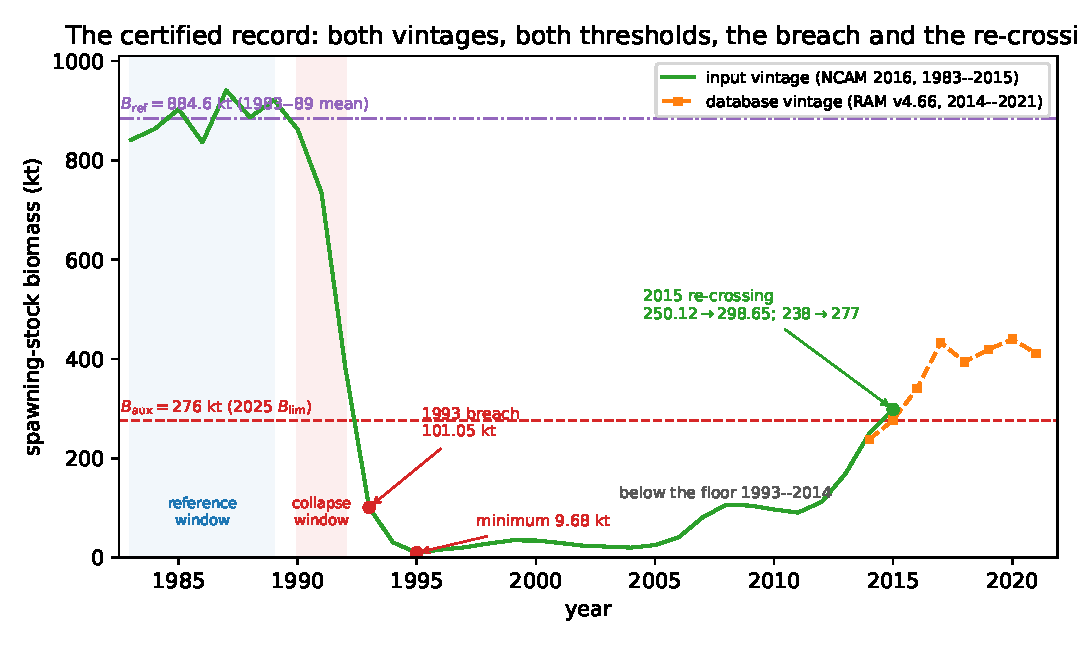
\includegraphics[width=0.96\linewidth]{figs_arv/fig_record.pdf}
\caption{The certified record, both vintages: the input vintage
(NCAM 2016, 1983--2015) and the database vintage (RAM v4.66, 2014--2021)
against the auxiliary floor ($276$ kt) and the reference point
($884.6$ kt); reference and collapse windows shaded; the 1993 breach
($101.05$ kt), the 1995 minimum ($9.68$ kt), the 22 consecutive
below-floor readings to 2014, and the 2015 re-crossing
($250.12 \to 298.65$; $238 \to 277$) as certified in the text.
Generated by the assertion script
\texttt{paper2\_arv\_record\_figure\_v1.py} (recompute-then-assert;
eleven exact checks against the locked files).}
\label{fig:record}
\end{figure}
\end{remark}

\begin{table}[t]
\centering
\scriptsize
\setlength{\tabcolsep}{2.8pt}
\caption{The certified quantities and their files. Computed in exact
rational arithmetic on the locked rows; displayed values rounded.}
\label{tab:summary}
\begin{tabular}{@{}l l l@{}}
\toprule
Quantity & Value & Source file \\
\midrule
Ref-window worst mult.\ (1986) & \(41800/45147\) & Table A2 \\
Collapse multipliers (1992, 1993) & \(0.520,\ 0.265\) & Table A2 \\
Collapse-step bracket bounds & \(0.7542,\ 0.3718\) & A2 $+$ T1 \\
Post-moratorium 2-yr factor & \(10105/968 \approx 10.44\) & Table A2 \\
Removals 1992, 1993 & \(40{,}956,\ 11{,}392\) & Table 1 (2025) \\
Removals 1994, 1995 & \(1{,}314,\ 413\) & T1 $=$ reconstr. \\
Survey index 1989, 1994 & \(2{,}127{,}417,\ 21{,}797\) & Survey T3 \\
Covariate 1990, 1991 & \(5783,\ 138\) & Capelin file \\
First below-floor reading & 1993 (\(101.05 < 276\)) & Table A2 \\
Cross-vintage 1993 levels & \(101.05\) vs \(79\) kt & A2 $+$ T17 \\
Outcome years 2016--2021 & \(340\)--\(440\) kt & DB extract \\
\bottomrule
\end{tabular}
\end{table}

\section{Delimitations}\label{scope}

Every arithmetic claim is a certificate about the realized rows of the
certified files --- not a forecast, not a stochastic model, and not a
counterfactual catch analysis. The bracket of
Lemma~\ref{lem:bracket} is an accounting decomposition: it removes the
realized removals from the per-capita rate under two extreme timing
conventions, and its harvest-free factor still conflates natural
mortality with recruitment --- the certified statement is that no
placement of the realized removals explains the decline, not that no
catch path could have. The biomass series are assessment outputs
(model-based), treated as the data of record with their published
uncertainty untouched; the exact arithmetic is exact on the published
point estimates, not a claim about the latent stock. The mortality
diagnostic is model-estimated given assumed catch, so the
mortality-crossing statement corroborates the regime reading without
independently certifying it; the survey index carries its own sampling
error and catchability assumptions, untouched here, and the
instrument--output divergence factor is certified as a difference of
rates, not attributed to a cause. The covariate series is
observed-years only; the contemporaneity statement is about certified
rows at annual resolution. Single stock; two vintages of one threshold
and one vintage of the reference point; no averaging beyond the
reference point's own construction.

\section{Verification methods}\label{methods}

Every number, fraction, inequality, power, ratio, bracket, and
temporal claim in this paper is regenerated by the accompanying script
in exact integer and rational arithmetic, standard library only,
directly from the locked files: the seven reference-window readings
with their six multipliers, exact mean
(\(\tfrac{44229}{50}\)), and minimum; the collapse-window and
connecting multipliers; the harvest-free brackets of
Table~\ref{tab:brackets} under both alignments, each upper bound
compared against unity by numerator--denominator comparison; the loss
factors \(\tfrac{352560}{40956}\) and \(\tfrac{280900}{11392}\) and
the removals share \(11392/280900\); the cross-file equality of the
1992--1995 removals rows and the 2015 row; the moratorium scale ratios
(\(\tfrac{231293}{1314}\) to \(\tfrac{268677}{413}\)); the
post-moratorium brackets and the two-year factor
\(\tfrac{10105}{968}\); the breach comparisons by integer
cross-multiplication (\(2021 \cdot 73451 < 7639 \cdot 27600\)) and the
first-below-floor pair with the 1992 intermediate; the cross-vintage
sign pattern, level factors, and implied-threshold range; the survey
factors and the divergence ratio; the covariate and mortality rows;
the threshold-discrimination below-sets; the sustained sixteenth-step
comparison; the two-vintage re-crossings, outcome values, and removals
range; and every headline number of this text asserted present
verbatim.

\section{Conclusion}\label{conclusion}

Applied to the public record of the Northern cod, the calculus
certifies the following. The collapse window's two annual steps are
harvest-free contractions under every timing convention the rows admit
(upper bounds \(0.754\) and \(0.372\)): no placement of the realized
removals --- which the year of the floor breach puts at \(4.06\%\) of
the stock's loss --- explains the decline, and under the moratorium's
own removals rows the non-fishing account drove a further certified
factor-of-\(10.4\) contraction to the series minimum. The reference
window's worst step and the two prelude steps do not admit that
reading: their brackets straddle unity, so the certified record
supports a typology (two harvest-free collapse steps inside a
fishing-era decline), not a blanket verdict about the decade. The
\(276\) kt auxiliary floor separates the eras without exception,
while the \(884.6\) kt reference point --- fixed at the window's own
mean --- has three of the seven window readings below it in sample
and separates nothing: a design property of mean-rule thresholds,
certified here on the readings themselves. The collapse is present in
the raw survey index at a certified factor of
\(\tfrac{21797}{2127417}\) over 1989--1994, falling \(2.6\) times
further over the common window than the assessment series it feeds;
the covariate crossing coincides with the mortality crossing at annual
resolution and leads the floor breach by two steps. Both assessment
vintages re-cross the floor at the 2015 reading and the outcome years
stay below half the reference point. The certificates are robust
where the bands allow them to be: on the reassessment vintage's
published 95\% bands, exactly the four collapse-era steps certify as
declines and the 1993 breach holds at the band's upper edge; and the
reference window's own profile (declines at horizons one to three,
growth at every horizon of four or more) delimits the sustained-rate
reading the record will bear --- as does the vintage's pre-window
record, which has the window open at \(28.3\%\) of the 1962 peak,
three years after a prior floor episode. These are exact statements about
published point estimates; their scope is the realized record, and
their monitoring content --- which instruments moved, when, relative to
which threshold --- is the applied content the obstruction calculus
prices.

\section*{References}

{\footnotesize
DFO (2016). Stock assessment of Northern cod (NAFO 2J3KL). \emph{Can.
Sci. Advis. Sec. Sci. Advis. Rep.} 2016/026.

Regular, P. et al. (2025). Northern cod (NAFO 2J3KL) reassessment.
\emph{DFO Can. Sci. Advis. Sec. Res. Doc.} 2025/048.

Schijns, R. et al. (2021). Reconstructing three centuries of fish and
fisheries catch in the Northwest Atlantic. \emph{ICES Journal of Marine
Science} 78, 2675--2684.

Abaee, A. (2026a). An obstruction calculus for viability under
incomplete observation. Submitted manuscript.

Abaee, A. (2026c). The Northern cod forecast ladder under a frozen
specification. Preprint.

Abaee, A. (2026d). Calibration data record, Northern cod (NAFO 2J3KL):
sources, cross-checks, and locked extracts. Preprint.

Hutchings, J.A., Myers, R.A. (1994). What can be learned from the
collapse of a renewable resource? Atlantic cod, Gadus morhua, of
Newfoundland and Labrador. \emph{Canadian Journal of Fisheries and
Aquatic Sciences} 51, 2126--2146.
}

\section*{Declarations}

\section*{Funding}
None.

\section*{Competing interests}
None.

\section*{Data availability}
All inputs are the archived public files of the calibration record
(wave-e-cod extracts and the record's CSV files), with primary sources
cited at archival time.

\section*{Code availability}
The verification script
\url{applied_regime_viability_v5_verification.py}
is publicly available at
\url{https://github.com/MIKEAA2020/general-sustainability} (folder
\texttt{arena agent 1/paper rewrites/latex}); it regenerates every
fraction, inequality, bracket, power, ratio, and temporal claim
verbatim from the locked files. The record figure is generated by
\texttt{paper2\_arv\_record\_figure\_v1.py} under the same discipline:
every plotted series value, threshold, crossing, and annotation is read
from the locked files and asserted exactly before the figure is written
(eleven checks).

\section*{AI declaration}
GLM (Z.ai), Qwen (Alibaba Cloud) and DeepSeek AI assisted with drafting
and iterative review. The author reviewed and edited outputs and takes
responsibility for the final work.

\end{document}
